Ce stage s'est déroulé en deux principales phases :
Une étape de developement durant laquelle des données et la fonction à apprendre ont été générées.
Et une étape plus appliquée durant laquelle une base de donnée réelle à été étudiée.\\


Afin d'implémenter informatiquement les concepts théoriques vus précédement, la librairie Keras à été utilisée\cite{keras}.
La partie sur les intégrales de choquet à été entierement recodée en python.
L'ensembe du code est bien évidement disponible gratuitement et sous licence libre sur github\cite{repoStage}.

\section{Keras}\label{sec:keras}
La librairie Keras est une interface Python/TensorFlow permetant de travailler avec des réseaux de neurones.
Cette librairie est très complète et permet de nombreuses choses.
Ici, on ne s'attardera que sur les fonctionnalitées principales,
a savoir la création d'un réseau simple,
la regression par \sgd\ et l'évaluation des performances.


Voici un exemple de réseau de neurone assez simple
qui vas essayer de deviner l'application linéaire suivante : $f(X) = 0.2x_1 + 0.8x_2$
\lstinputlisting[language=Python]{code/reseau1.py}
En executant ce code, on obtient:
\begin{lstlisting}
w0 : 0.19988934695720673
w1 : 0.8001111745834351
\end{lstlisting}
On peut donc bien voir que le réseau de neurones fonctionne et
réussit à apprendre des fonctions avec plusieurs paramètres.
Il est cependant assez embetant de toujours devoir faire appel a toutes ces fonctions.
Une librairie à alors été codée afin de simplifier son utilisation.
Elle pourra être appelée avec de nombreux paramtres qui seront abordés dans les parties suivantes.\\


On peut maintenant faire apprendre au réseau nimporte quelle application linéaire.
Par exemple la moyenne :

\begin{figure}[H]
    \center
    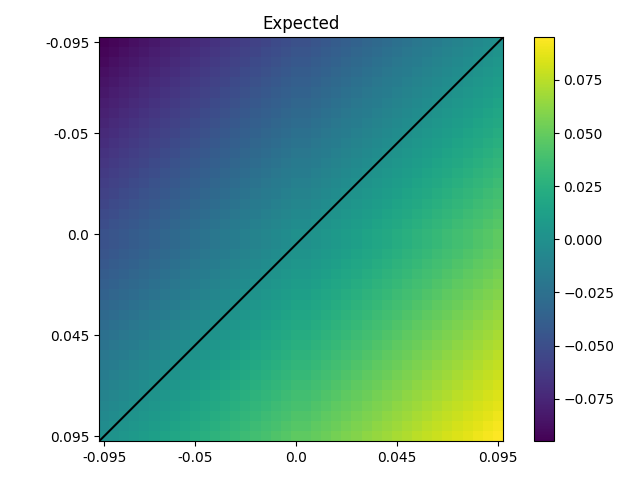
\includegraphics[height=\petit]{pict/moy/expected}
    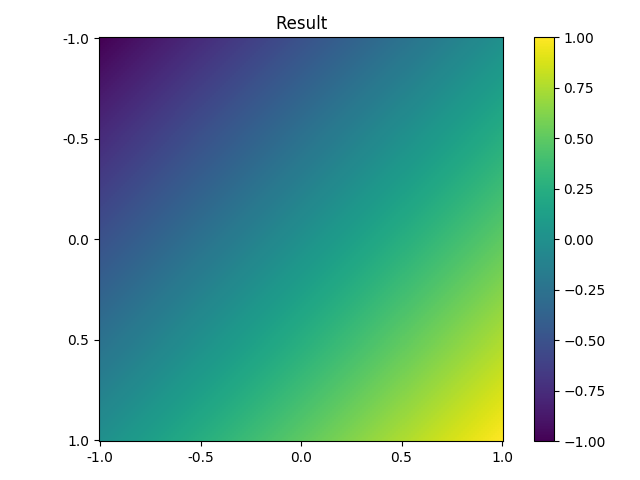
\includegraphics[height=\petit]{pict/moy/result}
	\caption{Apprentissage de la moyenne}
    \begin{center}
        \textit{
        A gauche, le résutltat atendu, a droite, celui renvoyé.\\
        $x_1$ en absice, $x_2$ en ordonées.
        }
    \end{center}
	\label{fig:moy}
\end{figure}
\vspace{-12pt}

On peut voir que la descente de gradients se fait a merveille.
Aucunes difference ne sont visibles : en effet les poids associés aux deux noeuds sont les suivants :
\begin{equation*}
    w_1 = 0.50000010
    \;\;\;\;\;\;\;\;\;
    w_2 = 0.50000024
\end{equation*}
On peut voir qu'aux aproximations processeur, les poids sont les bons pour faire la moyenne de deux nombres :
\begin{equation*}
    m =\frac{n_1 + n_2}{2} = 0.5 \times n_1 + 0.5 \times n_2
\end{equation*}


\section{Implementation d'un réseau de choquet}\label{sec:implementation-choquet}
Nous appellerons ici "réseau de choquet" un réseau de neurones ayant une architecture
adaptée a la regression d'une intégrale de choquet.
Comme vus precedement (\ref{subsec:intégrales-de-choquet}),
une fonction de choquet a une architecture complexe.
Voici l'architecture d'un réseau de choquet entierement générée par un réseau de neurones :

\begin{figure}[H]
    \center
    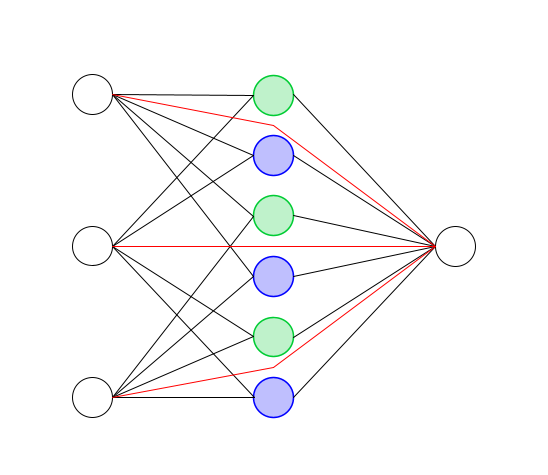
\includegraphics[height=\moyen]{pict/chnet1}
	\caption{Architecture d'un réseau de choquet}
	\label{fig:chnet1}
    \begin{center}
        \textit{
        En bleu, des neurone appliquant $\min(X)$, en vert $\max(X)$.
        }
    \end{center}
\end{figure}
\vspace{-12pt}
On peut voir que trois problemes non triviaux se posent :
\begin{itemize}
    \item Les neurones collorées n'appliquent pas une fonction simple.
    \item Les neurones ne sont pas reliés
\end{itemize}
